\chapter{Currents and circuits}
\section{Current}
\begin{definition}{Current}{current}
	Rate of flow of electric charge.
	\[I = \odv{q}{t} = \f{q_\text{tot}}{\Delta t}\:\text{for const.~current}\]
\end{definition}
Conventional current flows in the same direction as \hil{positive charges}.

The current flowing through a \bf{conductor} is
\[I = nAvq\]
\begin{itemize}
	\item \(n\) is the number of mobile charge carriers per unit volume\sidenote{intrinsic to the material}---number density [\unit{\per\cubic\metre}]
	\item \(A\) is the cross-sectional area
	\item \(v\) is drift velocity of charge carriers\sidenote{for the same material, \(v\propto\lf{1}{A}\)}
	\item \(q\) is the charge of one charge carrier
\end{itemize}

\section{V and emf}
\begin{definition}{Electromotive force}{emf}
	Energy converted \it{per unit charge} to electrical energy
	in driving charge around a complete circuit.
	\[\epsilon = \lf{W}{q}\]
\end{definition}
Emf is provided by an \hil{emf source} (e.g.~battery, generator),
where other forms of energy \(\to\) electrical energy.

\begin{definition}{Potential difference}{pd}
	Between two points, \underline{p.d.}~\(=\)~energy converted per unit
	charge from electrical energy \(\to\) other forms of energy,
	when charge is moved between the two points.
	\[\Delta V = \f{W}{q}\]
\end{definition}
P.d.~exists between two points/components in a circuit, where
electrical energy \(\to\) other forms of energy.

\section{Resistance}
\begin{definition}{Resistance}{resistance}
	\underline{Ratio} of p.d.~across a component to the current flowing through it. [\(\qty{1}{\ohm}=\qty{1}{\volt\per\ampere}\)]
	\[R = \f{V}{I} \neq \odv{V}{I}\]
	Not the gradient of a \(V\)-\(I\) graph.
\end{definition}

In circuits, \hil{effective resistance} is
\begin{align*}
	R_\text{eff} & = \sum_i R_i \quad\text{resistors \hil{in series}}                    \\
	R_\text{eff} & = \ab(\sum_i \f{1}{R_i})^{-1} \quad\text{resistors \hil{in parallel}}
\end{align*}

\begin{definition}{Ohm's law}{ohms-law}
	Provided that temperature/other physical conditions are constant,
	through a \it{metallic conductor},
	current flowing through it is directly proportional to the p.d.~across it.
\end{definition}

For a conductor of length \(L\), cross-sectional area \(A\), and resistivity\sidenote{intrinsic to the material} \(\rho\),
\[R = \f{\rho L}{A}\]

\section{Power}
\begin{definition}{Power}{e-power}
	Rate at which energy is converted from one form to another in a device
	\[P = IV \quad \text{(for all kinds of components)}\]
\end{definition}
For devices that \it{dissipate heat} (e.g.~resistors),
\[P = IV = I^2 R = \f{V^2}{R}\]

In practical applications, appliances should have \hil{high voltages}
so that the current is low (to produce the same power output).
Power loss due to Joule heating \(I^2R\) will be reduced.

\section{Circuits}
\subsection{\(I\)-\(V\) characteristics}
\begin{table}[htpb]
	\centering
	\begin{tabular}{r c l}
		\toprule
		component          & symbol                            & resistance...                                     \\
		\midrule
		metallic conductor & \tikz\draw(0,0) to[R] (1.5,0);    & is constant (\cref{def:ohms-law})                 \\
		filament lamp      & \tikz\draw(0,0) to[lamp] (1.5,0); & increases with temperature                        \\
		thermistor         & \tikz\draw(0,0) to[thR] (1.5,0);  & decreases with temperature                        \\
		diode              & \tikz\draw(0,0) to[Do] (1.5,0);   & forward biased: small; reverse biased: very large \\
		\bottomrule
	\end{tabular}
	\caption{Resistance of common components}
	\label{tab:component-resistance}
\end{table}
The components in \cref{tab:component-resistance} have various \(I\)-\(V\) characteristics (\term{memorise!}).
\begin{figure}[htpb]
	\centering
	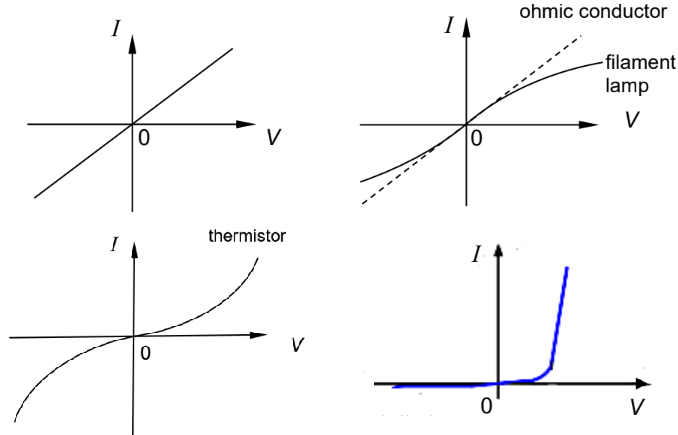
\includegraphics[width=0.8\textwidth]{assets/iv-characteristics.png}
	\caption{Some \(I\)-\(V\) characteristics}
	\label{fig:iv-characteristics}
\end{figure}
Explanations for common components
\begin{itemize}
	\item \bf{ohmic conductor} --- when \(T\) const, amplitude of lattice ion vibrations const. \(v\) const, \(R\) const.
	\item \bf{filament lamp}
	      \begin{itemize}
		      \item larger p.d., \(T\) increase.
		      \item amplitude of lattice ion vibrations increase, \(v\) decrease (given no change in \(n\)), \(R\) increase.
	      \end{itemize}
	\item \bf{thermistor} (negative temp.~coeff.)
	      \begin{itemize}
		      \item larger p.d., \(T\) increase
		      \item lattice vibrations increase, so hindrance to charge carrier flow increases (\(v\) decrease)
		      \item \it{but} thermistor also releases more charge carriers (\(n\) increase)
		      \item increase in \(n\) \it{larger than} the decrease in \(v\)
		      \item ratio \(\lf{V}{I}\) decrease, \(R\) decrease
	      \end{itemize}
	\item \bf{semiconductor diode} --- overly high reverse-biased p.d.~causes breakdown
\end{itemize}

\subsection{Internal resistance}
Emf sources have internal resistances \(r\), \cref{fig:int-resistance}.
\begin{marginfigure}
	\centering
	\begin{circuitikz}[scale=.8]
		\draw (0,0) to[R=$R$,v=$V_R$,i=$I$] (6, 0) -- (6,2) to[R=$r$] (3,2) to[battery1, l=\(\epsilon\), invert] (2,2) -- (0,2) -- (0, 0);
	\end{circuitikz}
	\caption{Internal resistance}
	\label{fig:int-resistance}
\end{marginfigure}
\begin{align*}
	\epsilon & = V_R + V_r   \\
	         & = I\ab(R + r) \\
	         & = V_R + Ir
\end{align*}

\subsection{Potential divider}
The p.d.~across any component is proportional to its resistance, within
the same closed loop.
\begin{marginfigure}
	\centering
	\begin{circuitikz}[scale=.8]
		\draw (6,2) to[battery1, l=$\epsilon$, invert] (0,2) to[short, -*, i=$I$] (0, 0) to[R=$R_1$, v=$V_1$] (2.5,0) to[short, -*, i=$I$] (3,0) to[R=$R_2$, v=$V_2$, i=$I$] (5.5,0) to[short,-*] (6,0) -- (6,2);
	\end{circuitikz}
	\caption{Potential divider}
	\label{fig:v-divider}
\end{marginfigure}
\begin{align*}
	I   & = \f{\epsilon}{R_1 + R_2}           \\
	V_1 & = IR_1 = \f{R_1}{R_1 + R_2}\epsilon \\
	V_2 & = IR_2 = \f{R_2}{R_1 + R_2}\epsilon \\
\end{align*}

\begin{marginfigure}
	\centering
	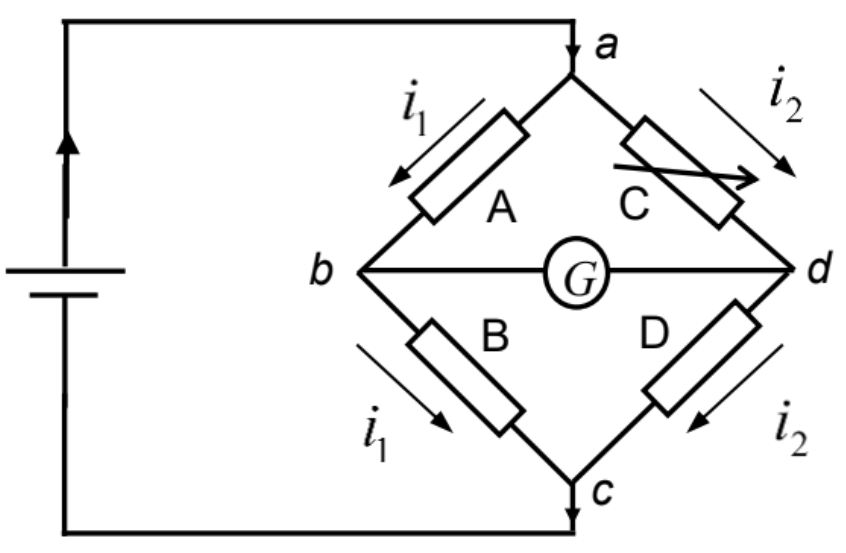
\includegraphics[width=\textwidth]{assets/wheatstone.png}
	\caption{Wheatstone bridge}
	\label{fig:wheatstone}
\end{marginfigure}
\begin{example}{}{wheatstone}
	The Wheatstone bridge (\cref{fig:wheatstone}) is useful for determining an unknown resistance \(R_C\).
	\begin{align*}
		V_{ab}                    & = V_{ad}        \\
		\implies i_1R_A           & = i_2R_C        \\
		V_{bc}                    & = V_{dc}        \\
		\implies i_1R_B           & = i_2R_D        \\
		\therefore\;\lf{R_A}{R_B} & = \lf{R_C}{R_D}
	\end{align*}
\end{example}

\section{Capacitors}
\begin{definition}{Capacitance}{capacitance}
	The ratio of the magnitude of the charge \(q\) to the potential difference across
	a capacitor \(V\). [\(\qty{1}{\farad} = \qty{1}{\coulomb\per\volt}\)]
	\[C = \f{q}{V}\]
\end{definition}
\hil{Effective capacitance} is
\begin{align*}
	C_\text{eff} & = \ab(\sum_i \f{1}{C_i})^{-1} \quad\text{capacitors \hil{in series}} \\
	C_\text{eff} & = \sum_i C_i \quad\text{capacitors \hil{in parallel}}
\end{align*}
The energy stored in a charged capacitor is
\[U = \f{qV}{2} = \f{q^2}{2C} = \f{CV^2}{2}\]

\subsection{Capacitor charging}
To charge a capacitor, an emf source is required.
\begin{marginfigure}
	\centering
	\begin{circuitikz}[scale=.8]
		\draw (0,0) to[R=$R$, v=$V_R$] (3,0) to[C=$C$,v=$V_C$] (6,0) to[nos] (6,2) to[battery,invert,l=$\epsilon$] (0,2) -- (0,0);
	\end{circuitikz}
	\caption{Capacitor charging}
	\label{fig:cap-charging}
\end{marginfigure}
\begin{align*}
	I & = I_0\exp\ab(-\f{t}{RC})        \quad\text{(charging current)} \\
	q & = q_0\ab[1-\exp\ab(-\f{t}{RC})]                                \\
	V & = V_0\ab[1-\exp\ab(-\f{t}{RC})] \quad\text{(across cap.)}      \\
\end{align*}
\begin{definition}{Time constant}{time-constant-charging}
	Time taken for charging current to fall to \(\lf{1}{e}\) of
	its initial value.
	\[\tau=RC\]
\end{definition}

\subsection{Capacitor discharging}
A charged \term{c}apacitor can discharge through a \term{r}esistor in a RC circuit.
\begin{equation*}
	J = J_0\exp\ab(-\f{t}{RC})\qquad J=I,q,V
\end{equation*}
\begin{marginfigure}
	\centering
	\begin{circuitikz}[scale=0.8]
		\draw (0,0) to[R=$R$, v=$V$, i=$I$] (6,0) to[nos] (6,2) to[C=$C$] (0,2) -- (0,0);
	\end{circuitikz}
	\caption{Capacitor discharging}
	\label{fig:cap-discharging}
\end{marginfigure}
\begin{definition}{Time constant}{time-constant-discharging}
	Time taken for \(I\), \(q\) or \(V\) to decrease to \(\lf{1}{e}\) of its initial value.
	\[\tau = RC\]
\end{definition}

\section{Alternating current}
\begin{definition}{Root mean square}{rms-current}
	The r.m.s.~value of an a.c.~is the \it{equivalent const.~d.c.} that
	dissipates the \it{same average power} in a given resistive load.
	\begin{align*}
		I_\text{r.m.s.} & = \sqrt{\ab<I^2>}                 \\
		\footnotesize
		\implies \ab<P> & = {I_\text{r.m.s.}}^2 R           \\
		                & = I_\text{r.m.s.} V_\text{r.m.s.}
	\end{align*}
\end{definition}
From an \(I\)-\(t\) graph (where \(I\) is periodic), we can get
\[I_\text{r.m.s.} = \sqrt{\ab<I^2>} = \sqrt{\f{1}{T}\int_{0}^{T}I^2\odif{t}}\]

For a \term{sinusoidal a.c.},
\begin{align*}
	I_\text{r.m.s.} & =\f{I_0}{\sqrt{2}} \\
	V_\text{r.m.s.} & =\f{V_0}{\sqrt{2}} \\
	\ab<P>          & = \f{1}{2}I_0V_0
\end{align*}

\subsection{Half-wave rectification}
Half-wave rectification converts an a.c.~supply into d.c.~output (\cref{fig:half-wave-rectification}).
\begin{figure}[htpb]
	\centering
	\begin{circuitikz}[scale=.8]
		\draw (0,0) to[sI] (0,2) to[empty diode, I=$I\ab(t)$] (4.5,2) to[R=$R$] (4.5,0) -- (0,0);
	\end{circuitikz}
	\label{fig:half-wave-rectification}
	\caption{Half-wave rectification}
\end{figure}

\Cref{fig:hwr-graph} shows a rectified sinusoidal a.c.
\begin{marginfigure}
	\centering
	\begin{tikzpicture}[
			declare function={
					halfwave(\x) = (\x<=pi) * (0.5*sin(deg(\x)))
					+ and(\x>pi, \x<=2*pi) * 0
					+ and(\x>2*pi, \x<=3*pi) * (0.5*sin(deg(\x-2*pi)))
					+ and(\x>3*pi, \x<=4*pi) * 0;
				}
		]
		\begin{axis}[
				width=\textwidth,
				xtick={0, 3.14159266, 6.28318531, 9.42477796, 12.566371},ytick={-.5, 0, .5},
				xticklabels={\(0\), \(\lf{T}{2}\), \(T\), \(\lf{3T}{2}\), \(2T\)},yticklabels={\(-I_0\), \(0\), \(I_0\)},
				xlabel=\(t\),ylabel=\(I\),
				ymin=-.6,
				ymax=.6,
				xmin=0,
				domain=0:12.7,
				samples=200,
				axis lines=middle,
			]
			\addplot[jiyopink, ultra thick] {0.5 * sin(deg(x)};
			\addplot[jiyoblue, ultra thick, smooth] {halfwave(x)};
			\legend{a.c., half-wave};
		\end{axis}
	\end{tikzpicture}
	\caption{Half-wave rectification}
	\label{fig:hwr-graph}
\end{marginfigure}

\begin{itemize}
	\item Diode is forward biased during one half-cycle, and reverse biased the next.
	\item When the rectifier is \it{forward biased}, current flows through the circuit, creating a p.d.~across \(R\).
	\item When the rectifier is \it{reverse biased}, little/no current flows, p.d.~\(= 0\).
\end{itemize}

After half-wave rectification,
\begin{align*}
	I_\text{r.m.s.} & = \lf{I_0}{2}    \\
	V_\text{r.m.s.} & = \lf{V_0}{2}    \\
	\ab<P>          & = \lf{I_0V_0}{4}
\end{align*}

\subsection{Full-wave rectification}
A full-wave rectifier uses the full a.c.~wave (\cref{fig:full-wave-rectifier}).
On the first half-cycle, \(D_{1,2}\) are forward biased and \(D_{3,4}\) reverse biased.
On the second half-cycle, \(D_{3,4}\) are forward biased and \(D_{1,2}\) reverse biased.
\begin{figure}
	\centering
	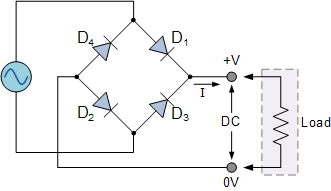
\includegraphics[width=.67\textwidth]{assets/full-wave-rectifier.png}
	\caption{Full-wave rectifier}
	\label{fig:full-wave-rectifier}
\end{figure}
\begin{marginfigure}
	\centering
	\begin{tikzpicture}
		\begin{axis}[
				width=\textwidth,
				xtick={0, 3.14159266, 6.28318531, 9.42477796, 12.566371},ytick={-.5, 0, .5},
				xticklabels={\(0\), \(\lf{T}{2}\), \(T\), \(\lf{3T}{2}\), \(2T\)},yticklabels={\(-I_0\), \(0\), \(I_0\)},
				xlabel=\(t\),ylabel=\(I\),
				ymin=-.6,ymax=.6,
				xmin=0,domain=0:12.7,
				samples=200,axis lines=middle,
			]
			\addplot[jiyopink, ultra thick] {0.5 * sin(deg(x)};
			\addplot[jiyoyellow, ultra thick, smooth] {0.5 * abs(sin(deg(x)};
			\legend{a.c., full-wave};
		\end{axis}
	\end{tikzpicture}
	\caption{Full-wave rectification}
	\label{fig:fwr-graph}
\end{marginfigure}
The effective frequency of the signal is doubled (\cref{fig:fwr-graph}).

\section{Kirchoff's laws (optional)}
\begin{enumerate}
	\item At a circuit junction, current arriving \(=\) current leaving\sidenote{\it{current arriving} as positive, \it{current leaving} as negative}.
	      \[\sum I = 0\]
	\item Around any closed loop, algebraic sum of emf \(=\) algebraic sum of current times resistance\sidenote{\(\epsilon\) and \(I\) are positive starting from the positive terminal}.
	      \[\sum_i \epsilon_i = \sum_i I_iR_i\]
\end{enumerate}

\section{Other examples}
\begin{example}{}{3-capacitors}
	What is the effective capacitance of this system?
	\begin{center}
		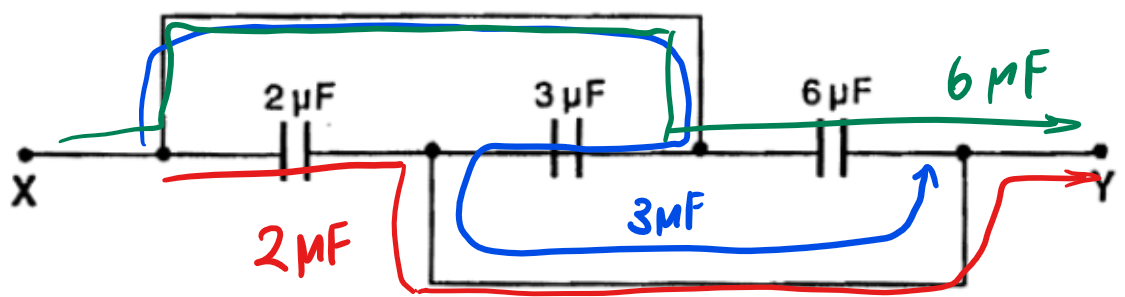
\includegraphics[width=0.7\textwidth]{assets/3-capacitors.png}
	\end{center}
	There are a total of 3 paths from X to Y. On each path,
	we encounter one of the three capacitors \(\implies\) capacitors are in parallel.
	\(C_\text{eff} = 2 + 3 + 6 = \qty{11}{\micro\farad}\).
\end{example}

\begin{example}{}{resistor-network}
	In this network of resistors, what is the p.d.~between X and Y?
	\begin{center}
		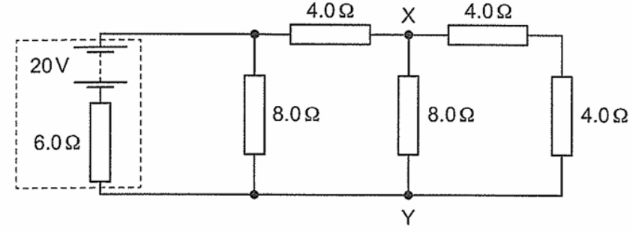
\includegraphics[width=.8\textwidth]{assets/r-network.png}
	\end{center}
	We can group the resistors together:
	\begin{center}
		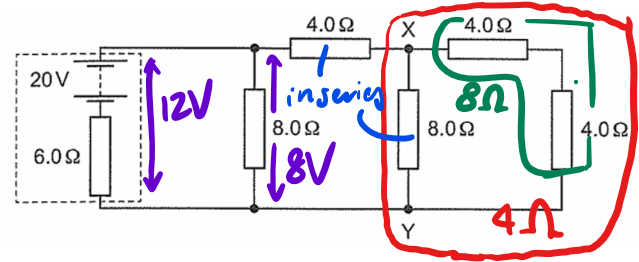
\includegraphics[width=.8\textwidth]{assets/r-network-redraw.png}
	\end{center}
	\begin{itemize}
		\item green: the two \(\qty{4.0}{\ohm}\) resistors combine to form an \(\qty{8}{\ohm}\) resistor
		\item red: combine the new \(\qty{8}{\ohm}\) resistor with the \(\qty{8.0}{\ohm}\) resistor across XY, to get a \(\qty{4}{\ohm}\) resistor
		\item purple: by potential divider, the p.d.~across the jumble of resistors is \(\lf{4}{\ab(4+6)}\cdot 20 = \qty{8}{\volt}\)
		\item blue: by potential divider, the \it{red resistor} and remaining \(\qty{4.0}{\ohm}\) resistor each have a p.d.~across them of \hil{\qty{4}{\volt}}
	\end{itemize}
\end{example}

\begin{example}{}{}
	Another network of resistors. What is the p.d.~between X and Y,
	and which point (X or Y) has greater potential?
	\begin{center}
		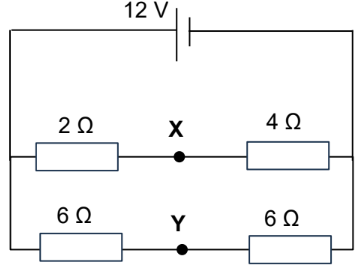
\includegraphics[width=.5\textwidth]{assets/rxy.png}
	\end{center}
	We \underline{start at \qty{0}{\volt} at the negative terminal}!
	\begin{center}
		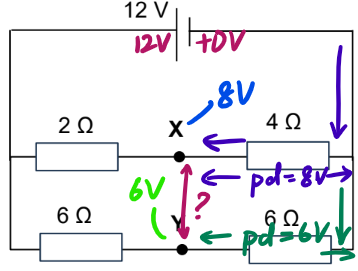
\includegraphics[width=.5\textwidth]{assets/rxy-redraw.png}
	\end{center}
	\begin{align*}
		V_X           & = \lf{4}{\ab(4+2)}\cdot 12=\qty{8}{\volt}\quad\text{(pot.~at a point)}       \\
		V_Y           & = \lf{6}{\ab(2\cdot 6)}\cdot 12= \qty{6}{\volt}\quad\text{(pot.~at a point)} \\
		\Delta V_{XY} & = 8-6=\hil{\qty{2}{\volt}}\quad\text{(p.d.!)}
	\end{align*}
	Point X is at higher potential.
\end{example}
